\appendix
\section{SPICE - ISO/IEC 15504}  \label{spice}
L'ISO/IEC 15504, noto come progetto \textbf{SPICE} (Software Process Improvement and Capability Evaluation), ha come obiettivo quello di sviluppare uno \glo{standard} che consenta valutazioni omogenee di organizzazioni software allo scopo di:
\begin{itemize}
	\item Identificare i punti forti, i punti deboli e i rischi delle metodologie utilizzate;
	\item Individuare le situazioni nelle quali le metodologie utilizzate permettono di raggiungere in maniera \glo{efficace} gli obiettivi prefissati.
\end{itemize}
Per effettuare la classificazione dei diversi processi, viene valutato e attribuito loro un livello di \textbf{Capability}, cioè la capacità di essere cognitivamente capace di raggiungere il suo scopo.
Ogni livello comprende degli attributi sui quali effettuare la valutazione.
I livelli considerati con i loro attributi sono i seguenti:
\begin{itemize}
	\item \textbf{Livello 0 Incomplete}: il processo non è implementato e non è in grado di raggiungere gli obiettivi;
	\item \textbf{Livello 1 Performed}: il processo è implementato e raggiunge gli obiettivi ma non è sottoposto a controlli costanti ai fini di correzione e miglioramento.
	Attributi associati:
	\begin{itemize}
		\item \textbf{Performance di processo (PP)}: numero degli obiettivi raggiunti.
	\end{itemize}
	\item \textbf{Livello 2 Managed}: il processo è gestito tramite pianificazione, controllo e correzione, l'output raggiunge gli obiettivi fissati.
	Attributi associati:
	\begin{itemize}
		\item \textbf{Gestione delle performance (PM)}: grado di organizzazione degli obiettivi fissati;
		\item \textbf{Gestione del prodotto di lavoro (WPM)}: grado di organizzazione dei prodotti rilasciati.
	\end{itemize}
	\item \textbf{Livello 3 Established}: esiste un'insieme di standard per il processo.
	Attributi associati:
	\begin{itemize}
		\item \textbf{Definizione di processo (PDEF)}: grado di adesione del processo agli standard;
		\item \textbf{Rilascio di processo (PDEP)}: grado di misura della garanzia di rilascio con reperibilità.
	\end{itemize}
	\item \textbf{Livello 4 Predictable}: il processo è istanziato coerentemente rispetto ai limiti previsti, è quantitativamente misurato per assicurarne il mantenimento delle performance.
	Attributi associati:
	\begin{itemize}
		\item \textbf{Misurazioni di processo (PME)}: misura con quanta \glo{efficacia} le metriche possono essere applicate al processo;
		\item \textbf{Controllo di processo (PC)}: grado di predicibilità dei risultati delle valutazioni.
	\end{itemize}
	\item \textbf{Livello 5 Innovating}: il processo migliora attraverso feedback quantitativi e gli standard sono adattati di conseguenza.
	Attributi associati:
	\begin{itemize}
		\item \textbf{Innovazione di processo (PI)}: misura quanto i cambiamenti attuati nel processo siano innovativi e positivi;
		\item \textbf{Ottimizzazione di processo (PO)}: misura quanto la curva di miglioramento sia lineare.
	\end{itemize}
\end{itemize}
Ogni attributo viene valutato e ad esso viene assegnato uno dei seguenti livelli, a seconda del grado di soddisfazione dello stesso:
\begin{itemize}
	\item \textbf{N not achieved}: 0\%-15\%, il processo non ha implementato l'attributo o presenta gravi lacune;
	\item \textbf{P partially achieved}: 16\%-50\%, il processo ha implementato l'attributo in modo sistematico ma risulta migliorabile o poco predicibile;
	\item \textbf{L largely achieved}: 51\%-85\%, il processo ha ampiamente implementato l'attributo ma il suo valore è poco uniforme rispetto alle altri parti del processo;
	\item \textbf{F fully achieved}: 86\%-100\%, il processo ha implementato completamente l'attributo ed è uniforme in ogni sua parte.
\end{itemize}

\newpage

\section{Ciclo di Deming - PDCA} \label{PDCA}
Il ciclo \textbf{PDCA} è un metodo iterativo con l'obiettivo di stabilire un modello per il miglioramento continuo dei processi ed essere garanzia di \glo{qualità} \glo{efficiente} e continuativa.
A tal fine si individuano quattro passaggi:
\begin{itemize}
	\item\textbf{Plan}: pianificazione, si esamina la situazione attuale al fine di determinare esattamente come raggiungere l'obiettivo;
	\item\textbf{Do}: implementazione, si procede a piccoli passi per realizzare quanto previsto durante la pianificazione;
	\item\textbf{Check}: verifica, vengono raccolti i risultati ottenuti e valutati rispetto agli obiettivi prefissati;
	\item\textbf{Act}: azione, i problemi e le cause identificate vengono risolte adattando quanto pianificato e infine attuato.
\end{itemize}
\begin{center}
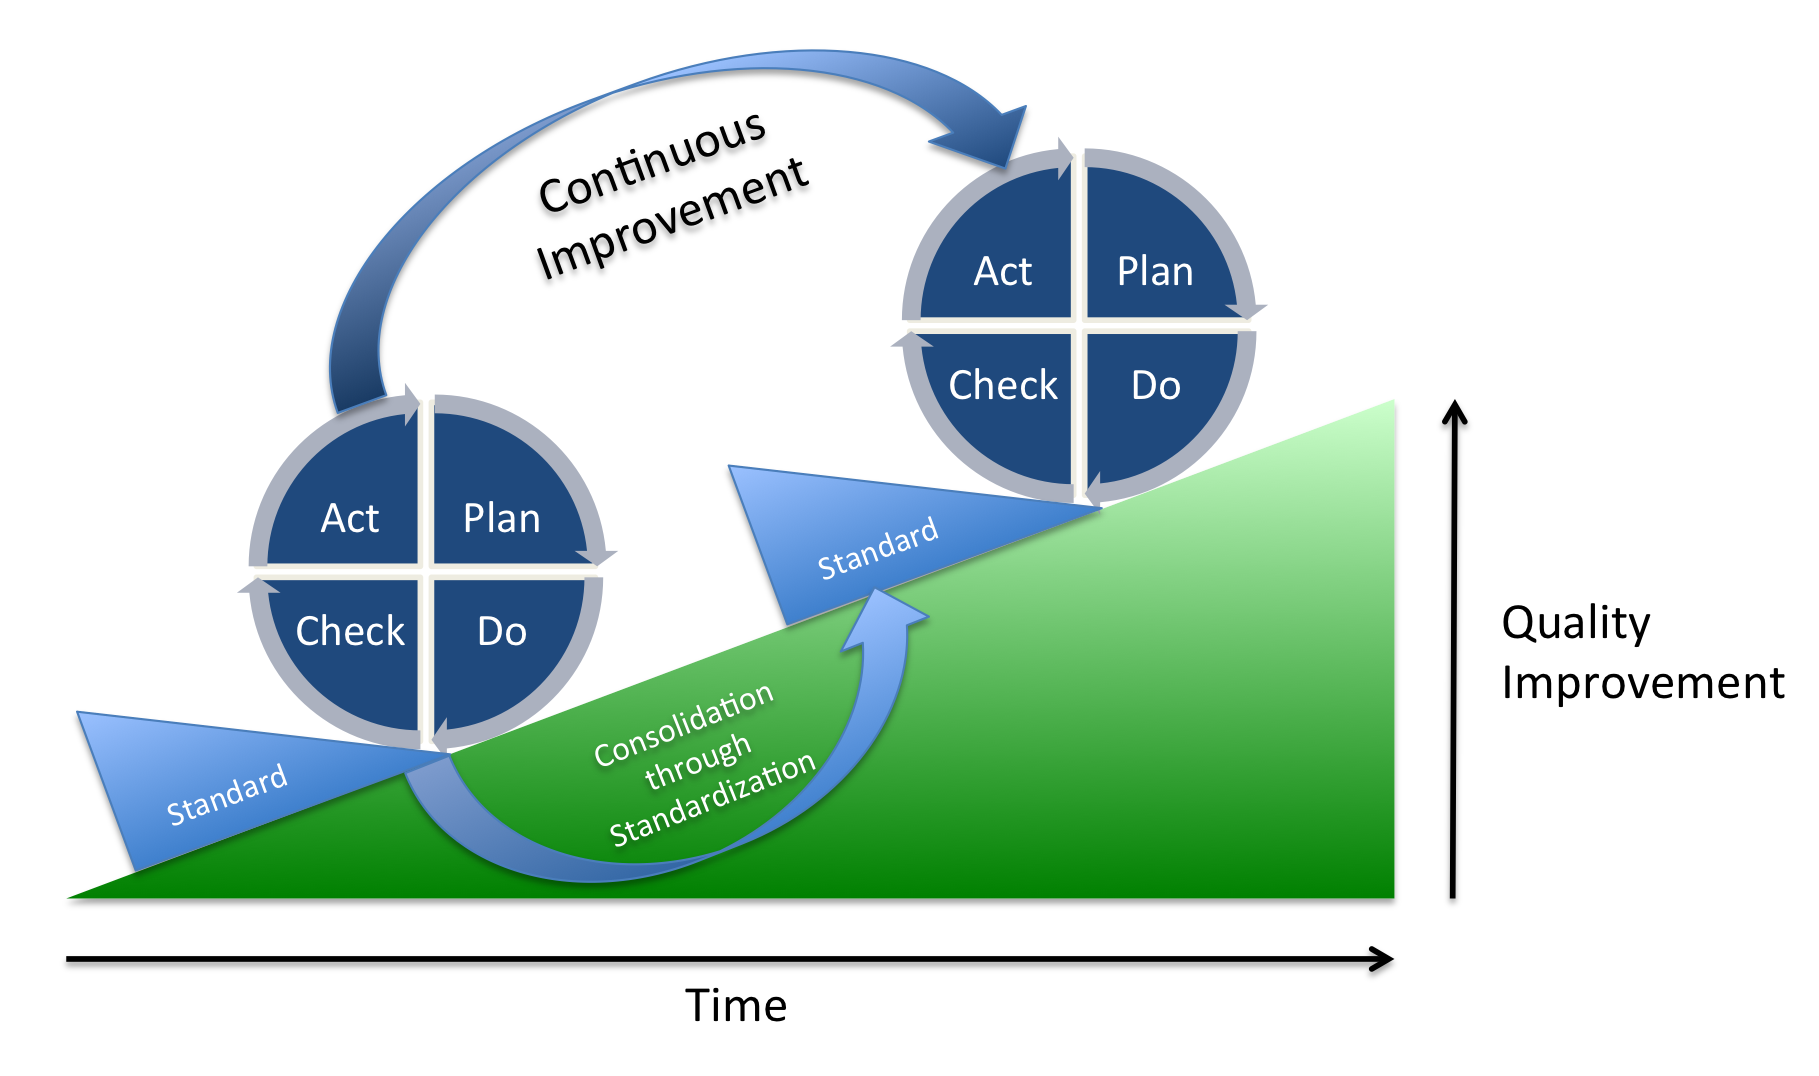
\includegraphics[scale=0.25]{Immagini/PDCA.png}
\captionof{figure}{Ciclo di Deming}
\end{center}

\newpage
\section{Standard ISO/IEC 9126}\label{9126}
L'ISO/IEC 9126 è uno standard internazionale per la valutazione della qualità del software, le norme presenti definiscono le caratteristiche che la determinano e propongono metriche per la misurazione.
Il modello di qualità software stabilito dallo standard considera sei caratteristiche principali da soddisfare, ovvero:
\begin{itemize}
	\item \textbf{Funzionalità};
	\item \textbf{Affidabilità};
	\item \textbf{Efficienza};
	\item \textbf{Usabilità};
	\item \textbf{Manutenibilità};
	\item \textbf{Portabilità}.
\end{itemize}
Le caratteristiche elencate possono essere misurate da \textbf{metriche esterne}, \textbf{metriche interne} e \textbf{metriche per la qualità d'uso}.
\paragraph*{Metriche Esterne}
Misurano i comportamenti del prodotto software rilevabili dai test, dall'operatività e dall'osservazione durante la sua esecuzione, in funzione degli obiettivi stabiliti.
\paragraph*{Metriche Interne}
Si applicano alla documentazione e al prodotto non eseguibile, ad esempio il codice sorgente, durante la progettazione e la codifica. Queste metriche misurano attributi interni del software e forniscono indicazioni sulle caratteristiche esterne del prodotto finale individuando problemi che potrebbero ridurne la qualità.
\paragraph*{Metriche per la qualità d'uso}
Misurano il grado con cui il prodotto software permette agli utenti di svolgere le proprie attività con efficacia, produttività, soddisfazione e sicurezza.

\subsection{Elenco delle metriche} \label{Metriche}
\subsubsection{Metriche per la qualità del processo}
\begin{itemize}
	\item  \hyperlink{MSoddRequisiti}{MPR01: Soddisfacimento requisiti obbligatori;}
	\item \hyperlink{MGulpease}{MPR02: Indice di Gulpease;}
	\item  \hyperlink{MOrtografia}{MPR03: Indice di correttezza ortografica;}
	\item  \hyperlink{MBC}{MPR04: Budget at Completion;}
	\item  \hyperlink{MACWP}{MPR05: Actual Cost of Work Performed;}
	\item  \hyperlink{MBCWP}{MPR06: Budget Cost of Work Performed;}
	\item  \hyperlink{MBCWS}{MPR07: Budget Cost of Work Scheduled;}
	\item  \hyperlink{MSV}{MPR08: Schedule Variance;}
	\item  \hyperlink{MBV}{MPR09: Budget Variance;}
	\item  \hyperlink{MProblemi}{MPR10: Indice di risoluzione dei problemi.} 
\end{itemize}

\subsubsection{Metriche per la qualità di prodotto}
\begin{itemize}
\item\hyperlink{MCImplementazione}{MPDS01: Completezza dell'implementazione;}
\item \hyperlink{MErrori}{MPDS02: Densità errori;}
\item\hyperlink{MFUtilizzo}{MPDS03: Facilità di utilizzo;}
\item\hyperlink{MFApprendimento}{MPDS04: Facilità di apprendimento;}
\item \hyperlink{MPGerarchia}{MPDS05:  Profondità della gerarchia;}
\item \hyperlink{MSFComprensione}{MPDS06: Facilità di comprensione;}
\item \hyperlink{MSFunzioni}{MPDS07: Semplicità delle funzioni;}
\item \hyperlink{MSC}{MPDS08: Semplicità delle classi.}
\end{itemize}